\documentclass[a4paper,12pt]{extarticle}
\usepackage[utf8]{inputenc}
\usepackage[francais]{babel}
\usepackage[T1]{fontenc}
\usepackage[pdftex]{graphicx}
\usepackage{url}
\usepackage{caption}
\usepackage{multirow}

\usepackage{fancyhdr}
\pagestyle{fancy}






\setlength{\parindent}{0cm}
\setlength{\parskip}{1ex plus 0.5ex minus 0.2ex}
\newcommand{\hsp}{\hspace{20pt}}
\newcommand{\HRule}{\rule{\linewidth}{0.5mm}}
%opening

\renewcommand{\headrulewidth}{1pt}
\fancyhead[L]{\leftmark}
\fancyhead[R]{LaTeX}

\renewcommand{\footrulewidth}{1pt}
\fancyfoot[C]{\textbf{page \thepage}} 




\begin{document}

\begin{titlepage}
  \begin{sffamily}
  \begin{center}

    % Upper part of the page. The '~' is needed because \\
    % only works if a paragraph has started.
    
\includegraphics[scale=1]{univangers.jpg}~\\[1.5cm]

    \textsc{\LARGE Université d'Angers}\\[2cm]

   

    % Title
    \HRule \\[0.4cm]
    { \huge \bfseries Virtualisation d'un équipement d'une classe mobile}{\bfseries  \\[0.4cm] }

    \HRule \\[2cm]
    

    % Author and supervisor
    \begin{minipage}{0.4\textwidth}
      \begin{flushleft} \large
        CHERRUAU \textsc{Anthony}\\
        FRESNEAU \textsc{Quentin}
        POUPELIN \textsc{Bastien}\\
        THEBAUDIN \textsc{Corentin}
      \end{flushleft}
    \end{minipage}
    

    \vfill
    \HRule\\[2cm]
    % Bottom of the page
    {\large 30 Mars 2017}

  \end{center}
  \end{sffamily}
\end{titlepage}
\clearpage

\tableofcontents

\clearpage



\section{Présentation de l'existant}

\subsection{Contexte}
\paragraph{}
Les étudiants de la faculté des sciences de l’université d’Angers disposent d’un chariot de 40 tablettes (Samsung Galaxy Tab 4) qui permet aux étudiants, lors de travaux pratiques d’Android, d’observer leurs applications sur un support concret autre qu’un émulateur.\\


Lors des préparations ou aux termes des contrôles continus de cette unité, l’enseignant peut avoir besoin de déposer des fichiers, les récupérer, contrôler les répertoires, accéder aux logs et installer des applications sur les tablettes.
A cet effet, un projet d’étudiant de L3 informatique a été mené en 2015 afin de répondre au cahier des charges précédemment cité. Jérôme FOURMOND et Florentin NOEL ont donc développé une application pour le chariot, une application pc et une application android.\\

L’application chariot permet d’exécuter des scripts qui s’appuient sur sur le kit de développement (SDK) d’android, ADB, et qui possède les même fonctionnalités sauf qu’une marque concrète des événements produits sur la machine est enregistrée.  Elle s'exécute directement dans un terminal et  se comporte comme un serveur, elle reçoit des messages simples et exécute des les scripts associés à ces messages. L’application sert de liaison entre les tablettes et l’application PC.\\

L’application PC est une application graphique qui permet une gestion simple des tablettes connectées grâce à son interface. Les scripts sont facile à exécuter et le résultat des commandes exécutées sont affichés. \\

L’application android permet à l’utilisateur de la tablette d’obtenir des informations sur son appareil via une interface graphique claire et de commander un nettoyage de l'appareil lors de sa prochaine connexion au chariot.\\

Actuellement le chariot de tablette est composé de la sorte. Nous avons un pc principal sous pfSense qui est relié vers le wifi et l’ethernet. Ensuite nous avons un pc vertical sous xubuntu qui permet de voir les tablettes et d’utiliser les script pour des fonctionnalités sur les tablettes. Les tablettes sont reliés à deux hub usb un pour le chariot du bas et un autre pour le chariot du haut. Ces hub sont ensuite reliés au Xubuntu.\\

Le schéma ci dessous représente le chariot actuelle :\\

\begin{center}
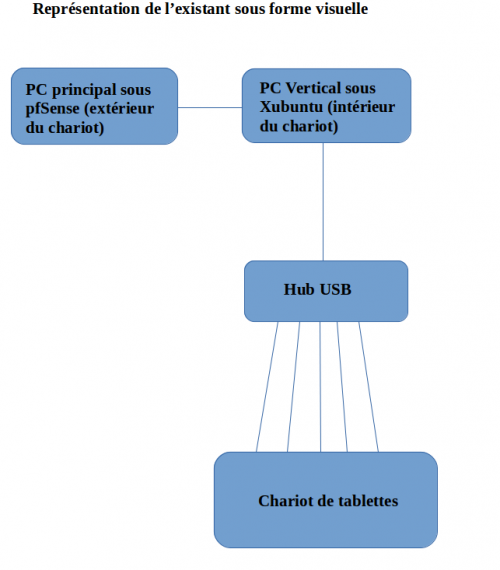
\includegraphics[scale=0.90]{representation_existant}
\end{center}

\clearpage
\subsection{Objectif du projet}

La finalité de ce projet est de permettre de n’avoir qu’un ordinateur contenant un hyperviseur de machines virtuelles, xenserver et deux machines virtuelle, le pfSense et le Xubuntu.
Cela permet de réduire le nombre de matériel requis pour le chariot. Au lieu d’avoir deux ordinateurs, tout est pilotables depuis un seul ordinateur et plus facile à gérer. De plus on peut prévoir de futures évolutions grâce à l’ajout de d’autres machines virtuelles au besoin.

Le schéma ci dessous représente le chariot désiré :\\

\begin{center}
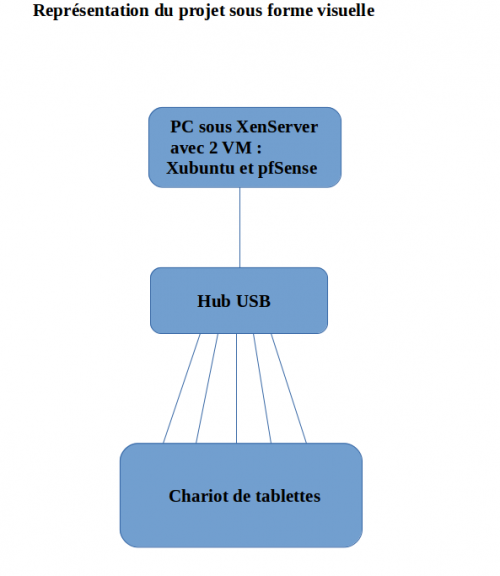
\includegraphics[scale=0.90]{representation_projet}
\end{center}

\clearpage
\section{Elaboration du projet}
\subsection{Partage du projet}

\paragraph{}
Concernant ce projet, nous avons séparé celui-ci de deux façons : la première étant l’installation et la seconde étant la recherche. En effet lors des phases d’installation, 
chacun cherchait de son cotés les différentes manières d’installer les différentes VMs. Suite à ces installations, nous étions souvent menés à chercher des solutions aux différents problèmes que l’on rencontrait (voir problèmes).

\subsection{Partage du travail(GANTT)}

cf annexe 1
Nous avons donc dû partager le travail. Pour cela nous avons donc défini des axes et avons réparti le travail. Pour cela nous avons un Gantt qui permet de voir ou l’on en ai et ce qu’il reste à faire.\\

\subsection{Matériel à disposition}

Au départ du projet plusieurs matériels ont été mis à notre disposition :
\begin{itemize}
\item Ordinateur portable HP EliteBook 8540w, i5M560, 4Go de ram
\item Un adaptateur HP usb/ethernet
\item Une clé usb 2.0 de 4Go
\item Une tablette Samsung galaxy tab
\item Une tablette Asus\\
\end{itemize}

Au fur et à mesure de l’avancement de notre projet nous avons rencontrés des problèmes matériels. C’est pour cela que de nouveaux matériels ont été mis à notre disposition :
\begin{itemize}
\item Ordinateur portable HP EliteBook 8560w, i7-2620M, 8Go
\item Un adaptateur Apple usb/ethernet
\item Un mini hub usb 3 port (brancher 2 tablettes)
\end{itemize}

\subsection{Réalisation du wiki}

L’une des consignes du projet était aussi de réaliser une page wikipédia contenant les étapes clés du projet, des tutoriels d’installation ou de résolution de problème et l’avancement de projet.
Notre tuteur nous a donc ouvert une section sur le wikipédia de l’université d’angers associant nos noms pour obtenir les droit d’écriture.\\

\url{http://wiki.info.univ-angers.fr/projets_etudiants:2017_l3pro_eg_virtualisation_classe_mobile}


\section{Mise en place de l'installation}
\subsection{XenServer}
\paragraph{Présentation\\}


Xen est un logiciel libre de virtualisation, ou plus précisément un hyperviseur de machine virtuelle basé sur centOS.\\

Xen permet d'exécuter plusieurs systèmes d'exploitation (et leurs applications) de manière isolée sur une même machine physique sur un grand nombre de plate-formes. Les systèmes d'exploitation invités partagent ainsi les ressources de la machine hôte.\\

Xen est un « paravirtualiseur » ou un « hyperviseur » de machines virtuelles. Les systèmes d'exploitation invités ont « conscience » du Xen sous-jacent, ils ont besoin d'être « portés » (adaptés) pour fonctionner sur Xen. Linux, NetBSD, FreeBSD, Plan 9 et GNU Hurd peuvent d'ores et déjà fonctionner sur Xen.\\

\paragraph{Dans le projet\\}

Pour débuter le projet, le choix de l’hyperviseur Xen à été fait en fonction des consignes notre tuteurs mais il aurait été possible d’utiliser d’autres logiciels libre gratuit équivalent tel que Proxmox. \\
Les premiers tests ont été réalisé avec la version 7.0 de XEN. L’installation se fait classiquement par le biais d’un ISO sur une clé USB bootable.

\begin{center}
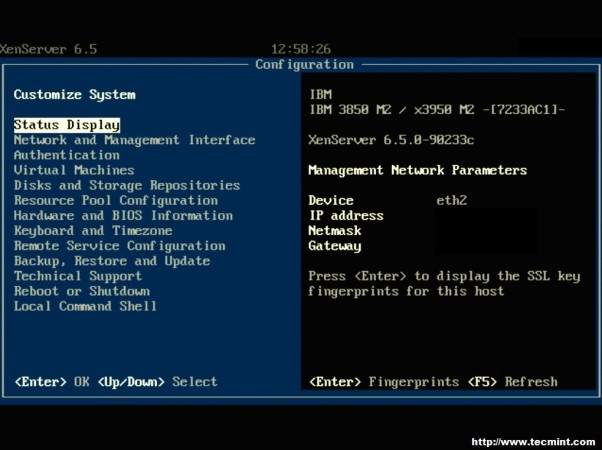
\includegraphics[scale=0.60]{xenserver18}\\
\end{center}

L’interface est plutôt sobre et ne permet de que quelques fonctionnalités simples comme le changement d’adresse IP ou le redémarrage de machines virtuelles.. Afin de pouvoir réaliser des opérations complexes comme la création d’une machine virtuelle, il faut utiliser les lignes de commandes ou un client externe dont nous parlerons dans la partie d de ce projet.\\

Les lignes de commande sont toutefois essentielles pour certaines fonctionnalités comme l’attribution d’un port USB à une machine virtuelle définit. Dans notre cas, la machine virtuelle Xubuntu devait pouvoir accéder à au moins 1 port USB pour être relié aux hub du chariot.

\subsection{PfSense}
\paragraph{Présentation\\}

PfSense est un routeur/pare-feu open source. Il utilise le pare-feu à états Packet Filter, des fonctions de routage et de NAT lui permettant de connecter plusieurs réseaux informatiques. Il comporte l'équivalent libre des outils et services utilisés habituellement sur des routeurs professionnels propriétaires. pfSense convient pour la sécurisation d'un réseau domestique ou de petite entreprise.


\paragraph{Dans le projet\\}

La machine virtuelle va nous permettre de faire le lien entre le wan et le lan. Le pfsense a deux interfaces réseaux : une qui est la carte réseau de l’ordinateur et l’autre qui est l’adaptateur ethernet/usb. Le pfsense va permettre que Xubuntu puisse avoir un lien vers l’extérieur et donc les tablettes auront accès au wan. 
PfSense est à la version 2.3.2 qui, au moment de l’installation, était la dernière version stable. Mais une nouvelle version est apparu entre temps la 2.3.3 mais nous n’avons pas mis à jour notre pfSense pour autant. Il y a donc une évolution de Pfsense possible. 

\begin{center}
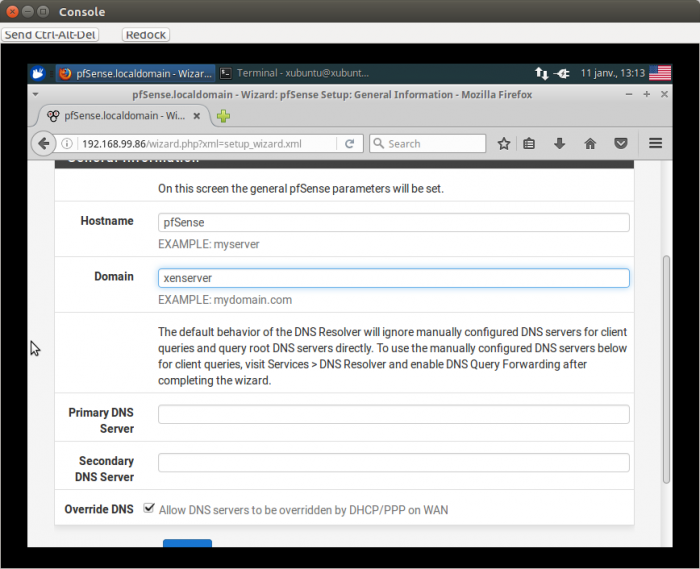
\includegraphics[scale=0.65]{pfsense}\\
\end{center}
\paragraph{}
PfSense peut être piloté par une interface web accessible depuis la machine virtuelle Xubuntu. La configuration s’est faite via le fichier de configuration de pfSense utilisé sur l’ancienne version du chariot.\\


\paragraph{}
\begin{table}[!h]
\begin{tabular}{|p{3cm}|p{3cm}|p{3cm}|p{3cm}|}
\hline
 & Configuration minimale & Configuration recommandée & Configuration choisie\\
\hline 
Processeur & 500 MHz & 1 GHz & 512 MHz\\
\hline
Mémoire vive & 512 Mo & 1 Go & 512 Mo \\
\hline
Stockage & >1 Go & & 15 Go \\
\hline
\end{tabular}
\caption{Configuration de pfsense}
\end{table}


\subsection{Xubuntu}
\paragraph{Présentation\\}

Xubuntu est un système d'exploitation libre de type GNU/Linux. C'est un projet issu de la Fondation Ubuntu utilisant l'environnement de bureau graphique Xfce à la place d'Unity. Le projet Xubuntu est une distribution Linux dérivée de Ubuntu, car tous deux partagent exactement la même base, des logiciels communs (Synaptic), les mêmes dépôts APT, le même nom de code et le même cycle de développement.


\paragraph{Dans le projet\\}

Nous utilisons dans notre versions la Xubuntu 16.04, Xenial Xerus qui est la dernière version de Xubuntu. C’est une version 64 bits puisque que l’ordinateur prêté est un 64 bits. De plus les scripts développés par les étudiants sont adaptés pour une machine en 64 bits.
Le choix de xubuntu est dû au fait que c’est un version plus légère de linux et cela permet sur une machine virtuelle d’économiser les ressources et d’avoir une machine virtuelle plus stable.
Le xubuntu va nous permettre de voir les tablettes et d’utiliser les script de gestion des tablettes. \\
Le choix de Xubuntu était imposé dès le début du projet car en prenant une Ubuntu par exemple, il y aurait eu  un problème sur le nombre de tablette détecté par ubuntu. La prise en charge de multiple matériel sur un usb est bloqué à sept sur Ubuntu d'où le choix de Xubuntu pour voir nos 40 tablettes. 
Pour le fonctionnement des scipt le kit de développement (SDK) d’android ADB a été ajouté à la machine.

\paragraph{\\}
\begin{table}[!h]
\begin{tabular}{|p{3cm}|p{3cm}|p{3cm}|p{3cm}|}

\hline
 & Configuration  minimale & Configuration recommandée & Configuration choisie\\
\hline 
Processeur & 750 MHz & 1,6 GHz & 1,6 MHz\\
\hline
Mémoire vive & 512 Mo & 2 Go & 2 Go \\
\hline
Stockage & 8 Go & 16 Go & 30 Go \\
\hline
\end{tabular}
\caption{Configuration de Xubuntu}
\end{table}

\subsection{OpenXenManager}

\paragraph{}
Travaillant sous Linux il nous fallait un logiciel pouvant se connecter à notre XenServer en ayant une interface graphique de nos machines virtuelles. Sous linux le seul logiciel est openXenManager qui est un logiciel officiel pour un XenServer. Ce dernier permet d’effectuer des actions sur l’hyperviseur et ses machines virtuelles. 
On peut par exemple créer des VMs, les stopper, les redémarrer. Une alternative à OpenXenManager existe sous Windows nommé XenCenter, on a dû aussi l’utiliser au cours du projet afin d’installer les tools manquants.

\begin{center}
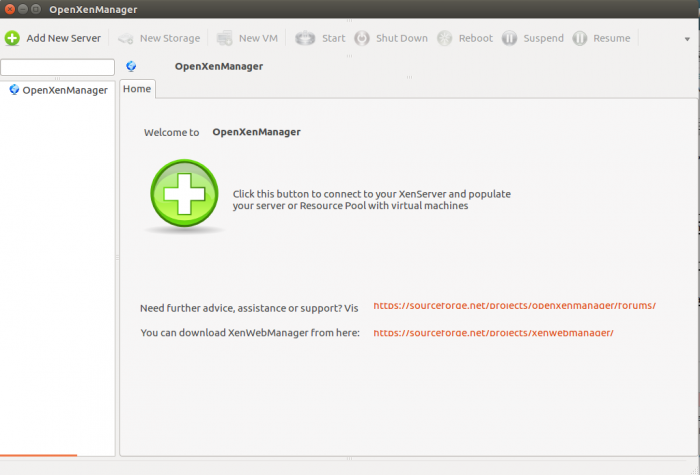
\includegraphics[scale=0.70]{openxenmanager}
\end{center}

\section{Etat final du projet}
\subsection{Présentation final du système}

\paragraph{}
Dans notre projet final nous avons un ordinateur tournant sous XenServer qui contient les machines virtuelles pfSense et Xubuntu. PfSense a deux cartes réseaux, celle de l’ordinateur pour le lan et l’adaptateur usb/ethernet pour le wan. Deux ports usb de l’ordinateur sont vu par le Xubuntu. En reliant l’ordinateur au chariot, les 40 tablettes ne pas forcément détectées par Xubuntu. Quand on branche les tablettes, sur chaque tablette un message s’affiche. 
Il faut l’accepter pour autoriser à ce qu’il y est une communication entre le xubuntu et les tablettes. Il faut aussi vérifier que le mode débogage soit bien actif sur les tablettes pour avoir ce message mais aussi pour pouvoir lancer les différents scripts. Nous pouvons utiliser le script des gestions tablettes pour vérifier le nombre de tablettes connectées et celles qui n’y sont pas. 
Le projet final est représenté par le schéma ci dessous :

\clearpage
\paragraph{Schéma du chariot détaillé}
\begin{center}
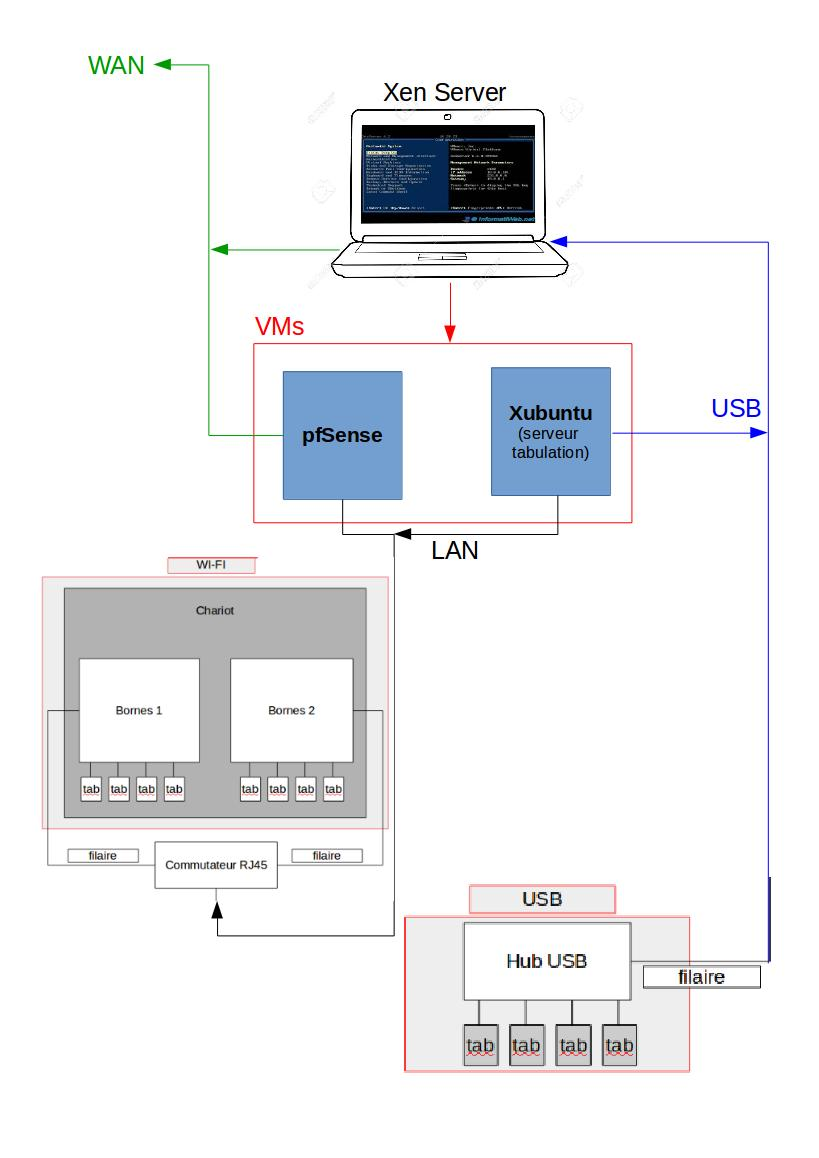
\includegraphics[scale=0.65]{chariot}\\
\end{center}

\subsection{Améliorations}

\paragraph{}
Il y a plusieurs axes d’améliorations possibles. 
Tout d’abord celui de gérer les bornes wifi depuis PfSense. Il y a déjà une configuration de faite mais pour mettre à jour une configuration de pfSense celui-ci doit avoir accès à internet. C’est pour cela que M.Girardeau a autorisé le pfSense à accéder au réseau de la fac sans authentification. Cela permettra donc de mettre à jour la configuration de pfSense et que les bornes wifi soit prises en compte. 
Ensuite pour avoir accès à toutes les machines sur un ordinateur il faudrait mettre XenServer en machine virtuelle sous Virtualbox par exemple et ensuite créer les machines virtuelles PfSense et Xubuntu depuis le xenserver. On pourrait ensuite accéder directement depuis le même ordinateur a toutes les machine virtuelles. Néanmoins, ce genre d’installation demanderait un ordinateur un peu plus puissant (surtout en terme de mémoire).

\section{Problèmes rencontrés}

\subsection{Problèmes matériels}

\paragraph{Reconnaissance de la tablette de test\\}
La tablette n’
ex :
était pas reconnu par la machine virtuelle Xubuntu.

Hypothèse :
\begin{itemize}
\item Protocole MTP (connexion des appareils android par USB) non géré par le noyau de linux de XEN
\item Le port USB n’est peut être pas monté \\
\end{itemize}

Solution :
Pour pouvoir utiliser les ports usb et que les tablettes soient reconnus sur la vm Xubuntu il faut que le port usb soit associé à la vm. 

lister les port USB et leur ID pour recuperer l'ID du port USB qui nous intéresse :
\begin{verbatim}
lspci
\end{verbatim}

lister les vm et leur UUID pour récupérer l’UUID qui nous intéresse :
\begin{verbatim}
xe vm-list
\end{verbatim}

Associer UUID et ID :
\begin{verbatim}
xe vm-param-set other-config:pci=”ID” uuid=”UUID”
\end{verbatim}
La machine Xubuntu detecte alors la tablette.



\paragraph{Reconnaissance de l'ensemble des tablettes\\}
Seulement 13 tablettes sur 40 de reconnu lors d'essai sur le chariot

Hypothèse :
\begin{itemize}
\item Test réalisé hors tension, peut être pas assez de courant pour pouvoir alimenté tous les ports USB ? 
\item Toutes les tablettes sont-elles en mode débogage ? 
\item Le noyau ou la configuration du noyau de l'ordinateur permet t'il de voir un nombre limité de tablettes ? \\
\end{itemize}

Test :
\begin{itemize}
\item Branchement de l'ordinateur sur secteur. NON CONCLUANT
\item Test de débranchement d'une tablette, une autre est prise en compte. NON CONCLUANT \\
\end{itemize}

Solution :
Problème de matériel : Alimentation fournit par le port USB pas assez importante. 
Nouvel ordinateur fournit.



\subsection{Problèmes logiciels}


\paragraph{Decouverte des ISOs lors de l'installation de VM\\}
Lors de l'installation des VMs via openXenManager, après transfert des ISOS, ceux-ci demeurent introuvable dans l'explorateur de fichiers.

Hypothèse :
\begin{itemize}
\item problème d'update de l'affichage des fichiers de OpenXenManager\\
\end{itemize}

Solution :
Transfert via SSH des ISOs puis reboot de XenServer.

\clearpage

\section{Conclusion}
blablablalbla

\section{Références}

Informations/Installation PfSense, Xubuntu et XenServer :

\url{https://fr.wikipedia.org/wiki/Xen}\\
\url{https://fr.wikipedia.org/wiki/Pfsense}\\
\url{http://www.sky-future.net/wp-content/uploads/2015/01/Installation+pfSense.pdf}\\
\url{https://services.renater.fr/ntp/serveurs_francais}\\

Installation/Lancement script Android :

\url{http://www.informatiweb-pro.net/virtualisation/1-citrix/15--citrix-xenserver-pci-passthrough--2.html}\\
\url{https://doc.ubuntu-fr.org/androiddebugbridge}\\
\url{https://launchpad.net/~nilarimogard/+archive/ubuntu/webupd8}\\

Réseau PfSense/XenServer/Xubuntu :

\url{https://support.citrix.com/article/CTX121615}\\

USB XenServer :

\url{https://medium.com/@alexander.bazhenov/\%D0\%BF\%D1\%80\%D0\%BE\%D0\%B1\%D1\%80\%D0\%BE\%D1\%81-usb-\%D1\%83\%D1\%81\%D1\%82\%D1\%80\%D0\%BE\%D0\%B9\%D1\%81\%D1\%82\%D0\%B2-\%D0\%B2-xenserver-50a9b4e8a80a#.icnppyde6}\\
\url{http://www.informatiweb-pro.net/virtualisation/1-citrix/15--citrix-xenserver-pci-passthrough--2.html}\\

Adaptateur ethernet :

\url{https://lists.xenproject.org/archives/html/xen-api/2013-07/msg00038.html}\\
\url{https://support.citrix.com/article/CTX121615}\\

\clearpage

\section{Annexes}

\begin{center}
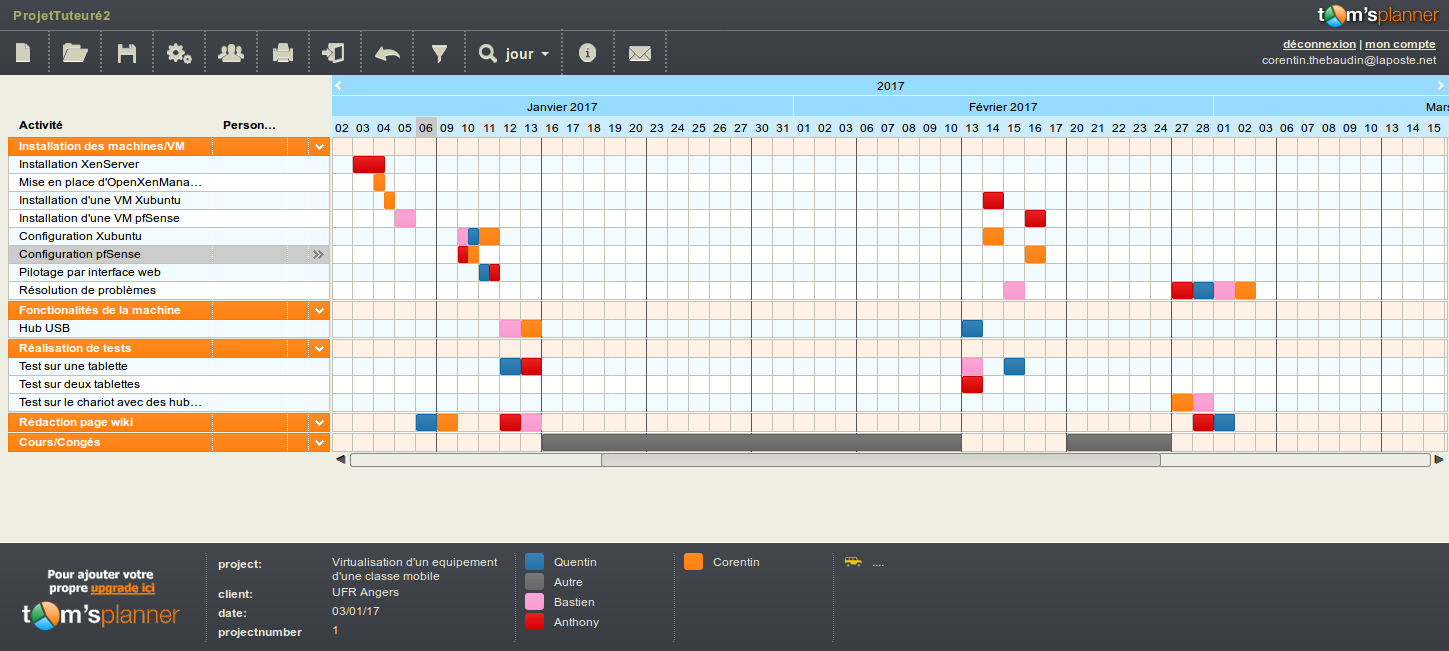
\includegraphics[scale=0.70, angle=270]{Gantt2}
\end{center}

\end{document}